\section{Proposal}

\begin{frame}
	\frametitle{BeeSafe project}
	
	I am also working on the \emph{BeeSAFE} project about ``\textbf{Learning for Multi-Robot Task Allocation}'' for
	the Sistemi Software Integrati (SSI) company.
	
	\vspace{0.4cm}
	
	\begin{block}{Objective}
		Developing a system that is able to autonomously coordinate a team of robots using learning techniques
	\end{block}
	
	\vspace{0.4cm}
	
	The project involves two main activities:
	
	\begin{enumerate}
		\item SLAM Multi-Robot
		\item \textbf{Multi-Robot Task Allocation}
	\end{enumerate}
\end{frame}

\begin{frame}
	\frametitle{Preliminary results}
	
	\vspace{0.3cm}
	
	We successfully developed a system to learn the best path for a robot, from a point A to a point B, in a
	simulative environment.
	
	\begin{center}
		\begin{tikzpicture}
			\node at (0,0) [draw=white,ultra thick,inner sep=0pt] {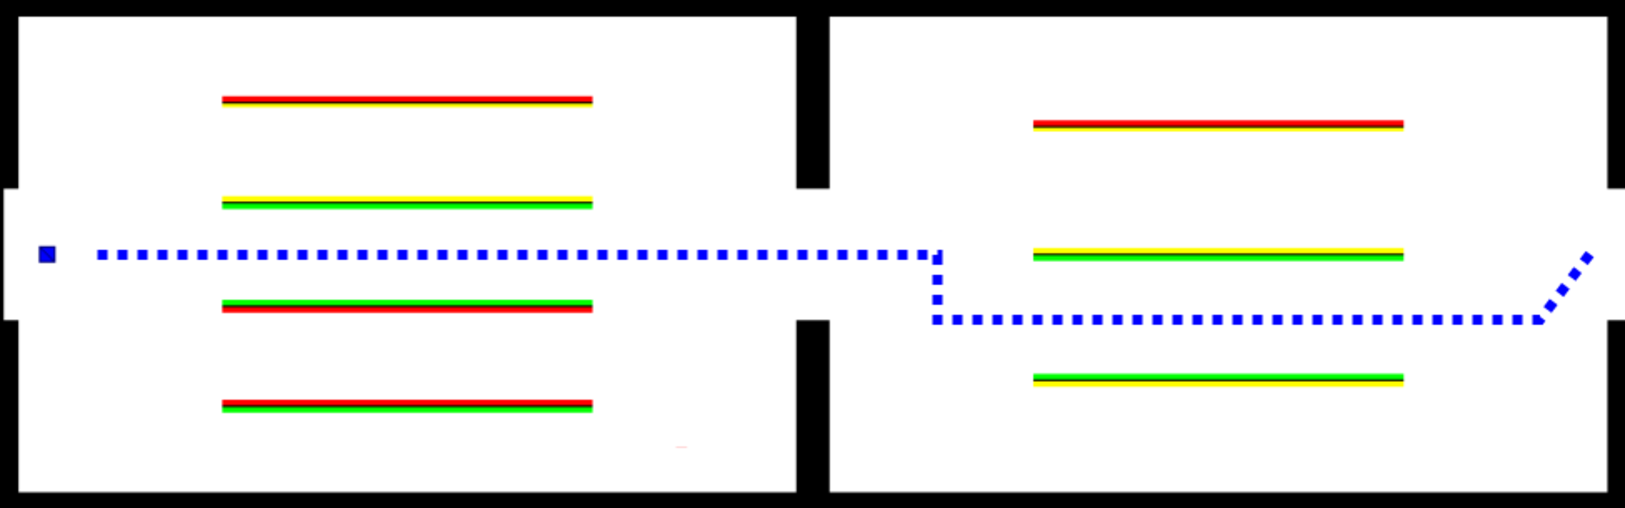
\includegraphics[scale=0.25]{images/BeeSAFE-1}};
		\end{tikzpicture}
	\end{center}
	
	\vspace{-0.1cm}
	
	\begin{columns}
		\column{0.6\textwidth}
		
		\centering
		The high level actions defined using the Petri Net Plans formalism.
		
		\vspace{-0.1cm}
		
		\begin{center}
			\begin{tikzpicture}
				\node at (0,0) [draw=white,ultra thick,inner sep=0pt] {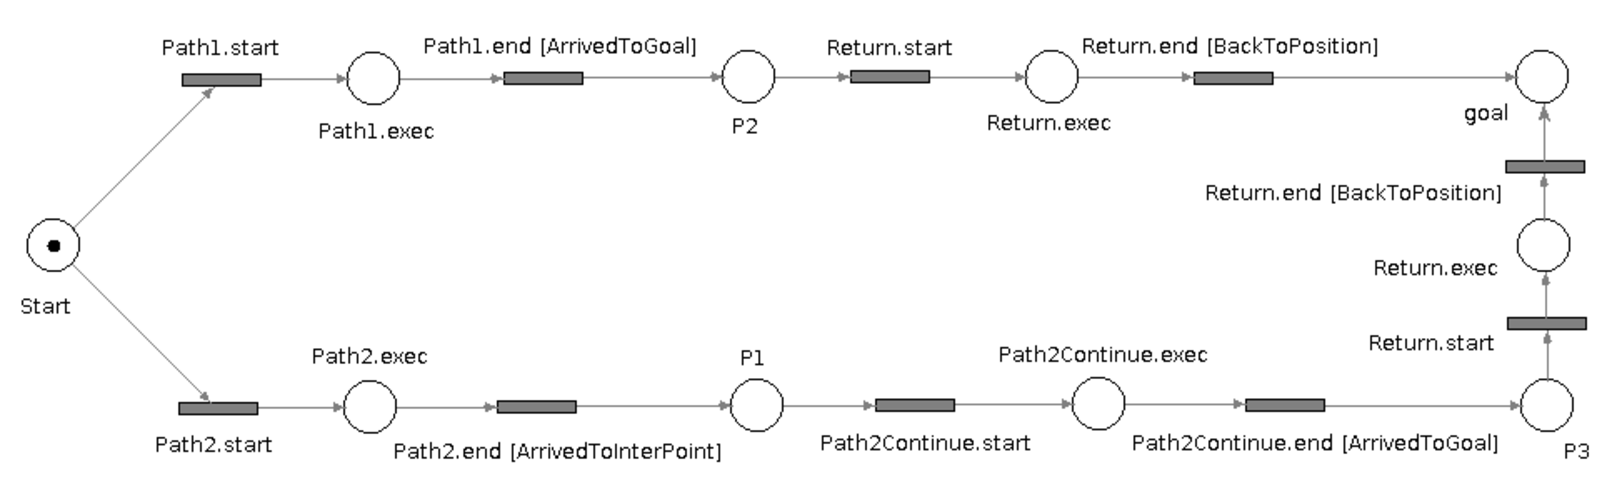
\includegraphics[height=2.1cm]{images/BeeSAFE-LearnPNP}};
			\end{tikzpicture}
		\end{center}
		
		\column{0.4\textwidth}
		
		\centering
		Learning applied on the \textbf{choices} points.
		
		\vspace{-0.1cm}
		
		\begin{center}
			\begin{tikzpicture}
				\node at (0,0) [draw=white,ultra thick,inner sep=0pt] {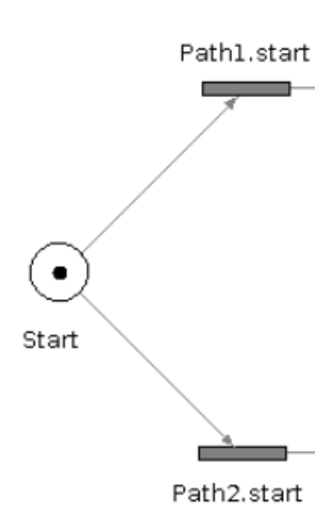
\includegraphics[height=2.1cm]{images/PNPChoice}};
			\end{tikzpicture}
		\end{center}
	\end{columns}
\end{frame}

\begin{frame}
	\frametitle{Learning best combined navigational abilities}
	
	\vspace{0.5cm}
	
	The experimental objective is to demonstrate that:

	\begin{enumerate}
		\item an \textbf{optimal solution} for a single robot can be different when introducing multiple robots
		\item \textbf{implicit coordination} among the robots in order to reach the best combined solution
	\end{enumerate}
	
	\vspace{0.2cm}
	
	A best combined path for two robots in the same environment.
	
	\vspace{-0.1cm}
	
	\begin{center}
		\begin{tikzpicture}
			\node at (0,0) [draw=white,ultra thick,inner sep=0pt] {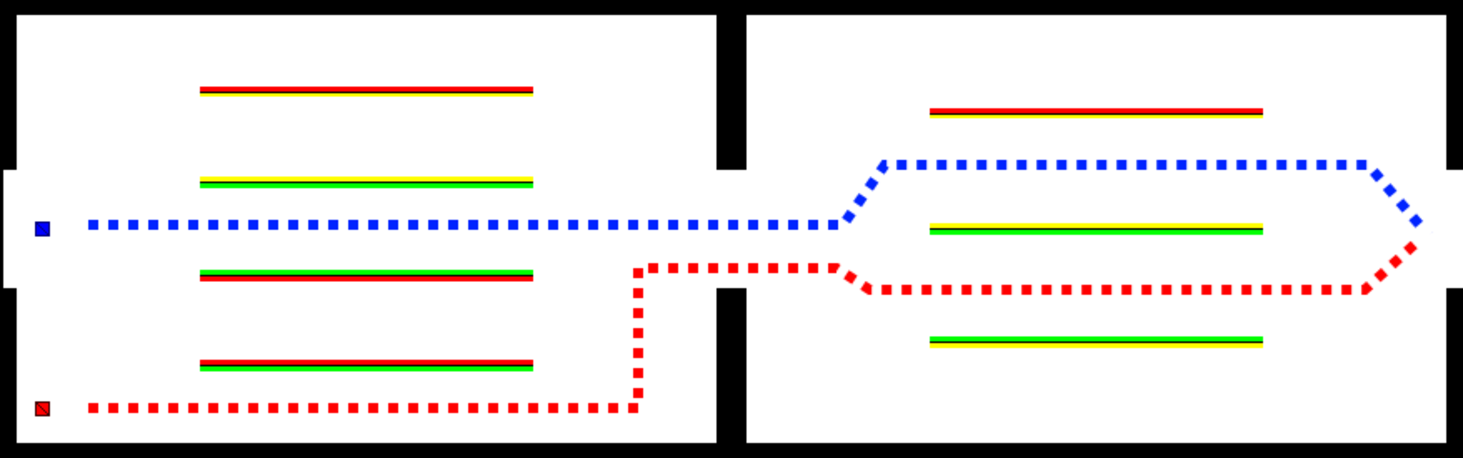
\includegraphics[scale=0.35]{images/BeeSAFE-2}};
		\end{tikzpicture}
	\end{center}
\end{frame}
